\hypertarget{introduction}{%
\section{Introduction}\label{introduction}}

Ecological networks are a useful way to think about ecological systems
in which species or organism interact (Delmas et al. 2018; Poisot,
Stouffer, and Kéfi 2016), and recently there has been an explosion of
interest in their dynamics across large temporal scales (Baiser et al.
2019; Tylianakis and Morris 2017), especially alongside environmental
gradients (Pellissier et al. 2017; Trøjelsgaard and Olesen 2016). As
ecosystems and climates are changing rapidly, ecologists realized that
networks are at risk or unravelling, being invaded by exotic species
that can destabilize them (Magrach et al. 2017; Strong and Leroux 2014),
or adopt entirely novel configurations (Hui and Richardson 2019; Guiden
et al. 2019). Simulation studies seem to suggest that knowing the shape
of the extant network is not sufficient (Thompson and Gonzalez 2017),
and that it needs to be supplemented by additional data on species
properties, climate, and climate projection.

This renewed interest in ecological networks has prompted several
methodological efforts. First, an expansion of the analytical tools to
study ecological networks and their variation in space (\textbf{REFS}).
Second, improvements in large-scale data-collection, through increased
adoption of molecular biology tools (\textbf{REFS}) and crowd-sourcing
of data collection (\textbf{REFS}). Finally, a surge in the development
of tools that allow to \emph{infer} species interaction
(Morales-Castilla et al. 2015) based on limited but complementary data
on existing network properties (Stock et al. 2017), species traits
(Gravel et al. 2013; Desjardins-Proulx et al. 2017; ~Brousseau, Gravel,
and Tanya Handa 2017; Bartomeus et al. 2016), and environmental
conditions (Gravel et al. 2018). These approaches tend to perform well
in data-poor environments (Beauchesne et al. 2016), and can be combined
through ensemble modeling or model averaging to generate possibly more
robust predictions (Pomeranz et al. 2018).

The common goal to these efforts is to facilitate the prediction of
network structure, both extant {[}Poisot, Gravel, et al. (2016);
\textbf{MARINE FOODWEB}{]} and future (Albouy et al. 2014), and to
appraise its possible variation in response to changes. All of these
developments also share the need to be supported by state of the art
data management: novel quantitative tools demand a higher volume of
network data; novel collection techniques demand powerful data
repositories; novel inference tools demand easier integration between
different types of data, including but not limited to interactions,
species traits, taxonomy, occurrences, and local bioclimatic conditions.

Poisot, Baiser, et al. (2016) -- overview of original DB + updates,
\textbf{TODO} map of networks + networks over time

\begin{itemize}
\tightlist
\item
  New data
\item
  number and amount of new information
\item
  web API for better data access, and two packages (one in Julia, the
  other in R) for accessing these data.
\item
  Mangal in its current form offers open network data that is ready to
  support synthesis at many scales.
\end{itemize}

Borrett, Moody, and Edelmann (2014) identified network ecology as one of
the fastest growing sub-field in the ecological sciences.

Synthesizing ecological data presents important challenges and also some
exciting opportunities. Mangal is well suited to offer such
opportunities in the study of ecological networks.

\begin{itemize}
\tightlist
\item
  A major challenge to ecological synthesis is generalizing from samples
  to the behaviour of ecological systems
\item
  two obstacles to such generalizing in ecological systems: data
  coverage and data quality

  \begin{itemize}
  \tightlist
  \item
    data coverage: are data collected from every relevant system?
  \item
    data quality: are data fit-for-purpose? Two particular aspects of
    quality

    \begin{itemize}
    \tightlist
    \item
      taxonomic resolution
    \item
      sampling effort
    \end{itemize}
  \end{itemize}
\end{itemize}

\textbf{Main question}, is the data fit for purpose, what can we do and
cannot do with it?

\hypertarget{global-trends-in-ecological-networks-description}{%
\section{Global trends in ecological networks
description}\label{global-trends-in-ecological-networks-description}}

\hypertarget{network-coverage-is-accelerating}{%
\subsection{Network coverage is
accelerating}\label{network-coverage-is-accelerating}}

\begin{figure}
\centering
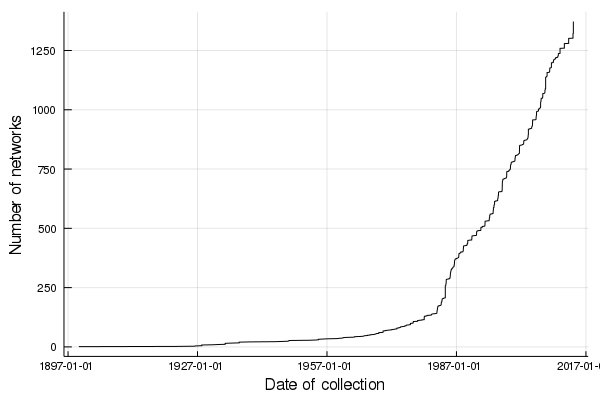
\includegraphics{figures/figure_01_a.png}
\caption{fig1\label{fig:temporal}}
\end{figure}

\hypertarget{different-interaction-types-have-been-studied-at-different-places}{%
\subsection{Different interaction types have been studied at different
places}\label{different-interaction-types-have-been-studied-at-different-places}}

\begin{figure}
\centering
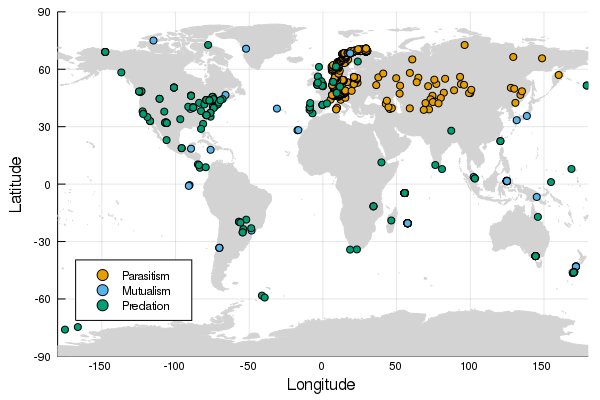
\includegraphics{figures/figure_01_c.png.png}
\caption{Each point on the map corresponds to a network with parasitic,
mutualistic, and predatory interactions. It is noteworty that the
spatial coverage of these types of interactions is uneven; the Americas
have almost no parasitic network, for example. Some places have barely
been studied at all, including Africa and Eastern Asia. This
concentration of networks around rich countries speaks to an inadequate
coverage of the diversity of landscapes on Earth.\label{fig:spatial}}
\end{figure}

\hypertarget{networks-follow-the-same-scaling}{%
\subsection{Networks follow the same
scaling}\label{networks-follow-the-same-scaling}}

Brose et al. (2004)

\begin{figure}
\centering
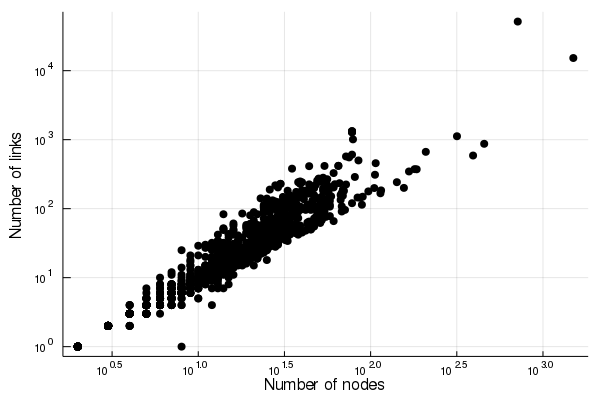
\includegraphics{figures/figure_01_b.png}
\caption{fig1 ref\label{fig:lssl}}
\end{figure}

\hypertarget{different-types-of-networks-have-been-studied-in-different-biomes}{%
\subsection{Different types of networks have been studied in different
biomes}\label{different-types-of-networks-have-been-studied-in-different-biomes}}

Whittaker (1962) suggested that natural communities can be partitioned
across biomes, largely defined as a function of their relative
precipitation and temperature; in \ref{fig:biomes}, we show that even
though networks, overall, capture the diversity of the
precipitation/temperature climate well, types of networks have been
studied in sub-spaces only. Specifically, parasitism networks have been
studied in colder and drier climates; mutualism networks in wetter
climates; predation networks display less of a bias.

\begin{figure}
\centering
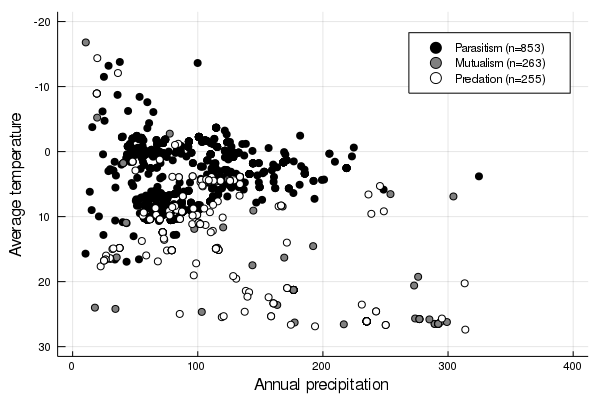
\includegraphics{figures/figure_02.png}
\caption{List of networks across biomes\label{fig:biomes}}
\end{figure}

\hypertarget{eccentricity-of-climate}{%
\subsection{Eccentricity of climate}\label{eccentricity-of-climate}}

\begin{figure}
\centering
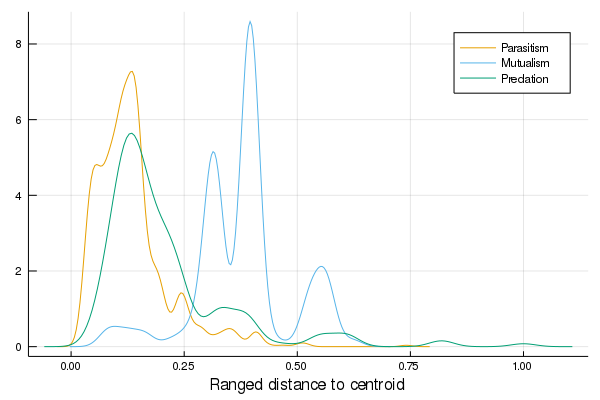
\includegraphics{figures/figure_05_b.png}
\caption{tk\label{fig:ecc}}
\end{figure}

\hypertarget{need-to-find-a-title}{%
\subsection{NEED TO FIND A TITLE}\label{need-to-find-a-title}}

Distance issues

\begin{figure}
\centering
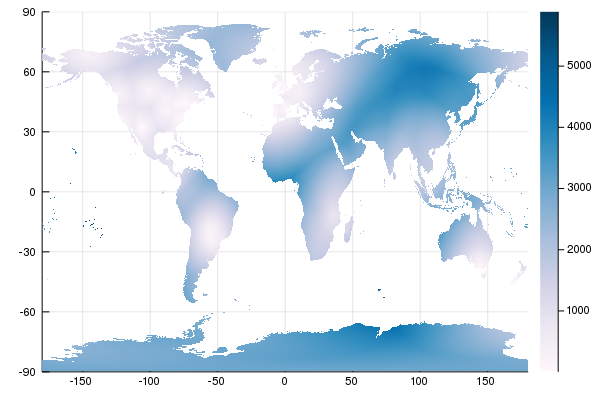
\includegraphics{figures/figure_03_a.png}
\caption{tk\label{fig:distance}}
\end{figure}

Climate analogue

\begin{figure}
\centering
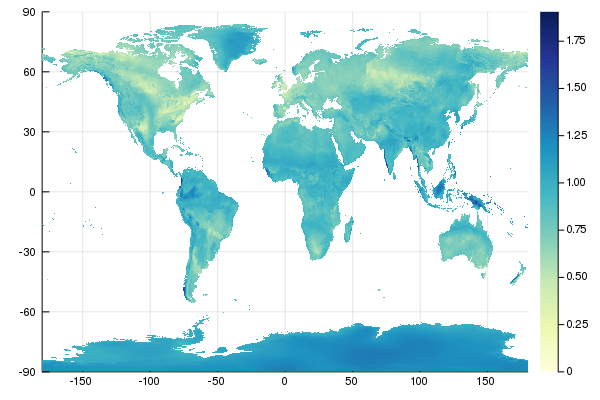
\includegraphics{figures/figure_03_b.png}
\caption{tk\label{fig:analog}}
\end{figure}

\hypertarget{conclusions}{%
\section{Conclusions}\label{conclusions}}

\hypertarget{reducing-uncertainty-through-analogues}{%
\subsection{reducing uncertainty through
`analogues'}\label{reducing-uncertainty-through-analogues}}

When we lack direct observation of a community, often we must resort to
the use of `analog' communities -- that is, communities which are
similar in space or environment which have been sampled.

\begin{itemize}
\tightlist
\item
  Communities may be similar in at least two ways -- close in space, or
  close in climate
\item
  similarity may result in some (?) similarity in network structure,
  even if species different.
\item
  Always some uncertainty in such comparisons
\item
  reflects the need for more data gathering, can be used to target
  efforts
\end{itemize}

\hypertarget{future-of-network-ecology}{%
\subsection{Future of network ecology}\label{future-of-network-ecology}}

Use this spatial gaps for sampling recommendations

\hypertarget{more-complete-analyses}{%
\subsection{more complete analyses}\label{more-complete-analyses}}

We have only shown some high-level summaries of the data here; many
possibilities remain.

\hypertarget{more-data-collection}{%
\subsection{more data collection}\label{more-data-collection}}

We have demonstrated the considerable coverage of Mangal; however, our
summary also highlights important data-collection needs. In particular,
we need better information about (mutualists, desert food webs?)

\hypertarget{active-development-and-data-contribution}{%
\subsection{Active development and data
contribution}\label{active-development-and-data-contribution}}

This is an open-source project: all data and all code supporting this
are available on the Mangal project GitHub organization. Our hope is
that the success of this project will encourage similar efforts within
other parts of the ecological community. In addition, we hope that this
project will encourage the recognition of the contribution that software
creators make to ecological research.

\hypertarget{data-quality-sampling-effort-and-taxonomy}{%
\subsection{Data quality: sampling effort and
taxonomy}\label{data-quality-sampling-effort-and-taxonomy}}

Sampling effort and taxonomic detail are two very challenging but
important part of any ecological dataset. The datasets in Mangal
represent some of the most detailed studies of ecological networks
available. * measures of network structure may be particularly sensitive
to the amount of sampling effort * repeat sampling may be necessary to
capture a ``saturation'' of interactions. * we present some
visualization of the sampling coverage of Mangal {[}tk{]} * High
taxonomic resolution is difficult to achieve in ecology, especially
depending on the sampling method used (e.g.~gut contents vs
observations). We present a breakdown of the taxonomic resolution of
Mangal. * Ecological networks occur in various kinds, but they are not
all equally well sampled. We present a breakdown of the number of
parasitic, mutualistic and predator-prey networks sampled in Mangal

\hypertarget{references}{%
\section*{References}\label{references}}
\addcontentsline{toc}{section}{References}

\hypertarget{refs}{}
\leavevmode\hypertarget{ref-AlboVele14}{}%
Albouy, Camille, Laure Velez, Marta Coll, Francesco Colloca, François Le
Loc'h, David Mouillot, and Dominique Gravel. 2014. ``From Projected
Species Distribution to Food-Web Structure Under Climate Change.''
\emph{Global Change Biology} 20 (3): 730--41.
\url{https://doi.org/10.1111/gcb.12467}.

\leavevmode\hypertarget{ref-BaisGrav19}{}%
Baiser, Benjamin, Dominique Gravel, Alyssa R. Cirtwill, Jennifer A.
Dunne, Ashkaan K. Fahimipour, Luis J. Gilarranz, Joshua A. Grochow, et
al. 2019. ``Ecogeographical Rules and the Macroecology of Food Webs.''
\emph{Global Ecology and Biogeography} 0 (0).
\url{https://doi.org/10.1111/geb.12925}.

\leavevmode\hypertarget{ref-BartGrav16}{}%
Bartomeus, Ignasi, Dominique Gravel, Jason M. Tylianakis, Marcelo A.
Aizen, Ian A. Dickie, and Maud Bernard-Verdier. 2016. ``A Common
Framework for Identifying Linkage Rules Across Different Types of
Interactions.'' \emph{Functional Ecology} 30 (12): 1894--1903.
\url{https://doi.org/10.1111/1365-2435.12666}.

\leavevmode\hypertarget{ref-BeauDesj16}{}%
Beauchesne, David, Desjardins-Proulx, Philippe Archambault, and
Dominique Gravel. 2016. ``Thinking Outside the Box--Predicting Biotic
Interactions in Data-Poor Environments.'' \emph{Vie et Milieu-Life and
enVironment} 66 (3-4): 333--42.

\leavevmode\hypertarget{ref-BorrMood14}{}%
Borrett, Stuart R., James Moody, and Achim Edelmann. 2014. ``The Rise of
Network Ecology: Maps of the Topic Diversity and Scientific
Collaboration.'' \emph{Ecological Modelling} 293 (December): 111--27.
\url{https://doi.org/10.1016/j.ecolmodel.2014.02.019}.

\leavevmode\hypertarget{ref-BrosOstl04}{}%
Brose, Ulrich, Annette Ostling, Kateri Harrison, and Neo D. Martinez.
2004. ``Unified Spatial Scaling of Species and Their Trophic
Interactions.'' \emph{Nature} 428 (6979): 167--71.
\url{https://doi.org/10.1038/nature02297}.

\leavevmode\hypertarget{ref-BrouGrav17}{}%
Brousseau, Pierre-Marc, Dominique Gravel, and I. Tanya Handa. 2017.
``Trait-Matching and Phylogeny as Predictors of Predator-Prey
Interactions Involving Ground Beetles.'' \emph{Functional Ecology},
July. \url{https://doi.org/10.1111/1365-2435.12943}.

\leavevmode\hypertarget{ref-DelmBess18}{}%
Delmas, Eva, Mathilde Besson, Marie-Hélène Brice, Laura A. Burkle,
Giulio V. Dalla Riva, Marie-Josée Fortin, Dominique Gravel, et al. 2018.
``Analysing Ecological Networks of Species Interactions.''
\emph{Biological Reviews}, June, 112540.
\url{https://doi.org/10.1111/brv.12433}.

\leavevmode\hypertarget{ref-DesjLaig17}{}%
Desjardins-Proulx, Philippe, Idaline Laigle, Timothée Poisot, and
Dominique Gravel. 2017. ``Ecological Interactions and the Netflix
Problem.'' \emph{PeerJ} 5 (e3644).
\url{https://doi.org/10.7717/peerj.3644}.

\leavevmode\hypertarget{ref-GravBais18}{}%
Gravel, Dominique, Benjamin Baiser, Jennifer A. Dunne, Jens-Peter
Kopelke, Neo D. Martinez, Tommi Nyman, Timothée Poisot, et al. 2018.
``Bringing Elton and Grinnell Together: A Quantitative Framework to
Represent the Biogeography of Ecological Interaction Networks.''
\emph{Ecography} 0 (0). \url{https://doi.org/10.1111/ecog.04006}.

\leavevmode\hypertarget{ref-GravPois13}{}%
Gravel, Dominique, Timothée Poisot, Camille Albouy, Laure Velez, and
David Mouillot. 2013. ``Inferring Food Web Structure from Predator-Prey
Body Size Relationships.'' Edited by Robert Freckleton. \emph{Methods in
Ecology and Evolution} 4 (11): 1083--90.
\url{https://doi.org/10.1111/2041-210X.12103}.

\leavevmode\hypertarget{ref-GuidBart19}{}%
Guiden, Peter W., Savannah L. Bartel, Nathan W. Byer, Amy A. Shipley,
and John L. Orrock. 2019. ``Predator--Prey Interactions in the
Anthropocene: Reconciling Multiple Aspects of Novelty.'' \emph{Trends in
Ecology \& Evolution} 0 (0).
\url{https://doi.org/10.1016/j.tree.2019.02.017}.

\leavevmode\hypertarget{ref-HuiRich19}{}%
Hui, Cang, and David M. Richardson. 2019. ``How to Invade an Ecological
Network.'' \emph{Trends in Ecology \& Evolution} 34 (2): 121--31.
\url{https://doi.org/10.1016/j.tree.2018.11.003}.

\leavevmode\hypertarget{ref-MagrHolz17}{}%
Magrach, Ainhoa, Andrea Holzschuh, Ignasi Bartomeus, Verena Riedinger,
Stuart P. M. Roberts, Maj Rundlöf, Ante Vujić, et al. 2017.
``Plant-Pollinator Networks in Semi-Natural Grasslands Are Resistant to
the Loss of Pollinators During Blooming of Mass-Flowering Crops.''
\emph{Ecography}, February, n/a--n/a.
\url{https://doi.org/10.1111/ecog.02847}.

\leavevmode\hypertarget{ref-MoraMati15}{}%
Morales-Castilla, Ignacio, Miguel G. Matias, Dominique Gravel, and
Miguel B. Araújo. 2015. ``Inferring Biotic Interactions from Proxies.''
\emph{Trends in Ecology \& Evolution}.

\leavevmode\hypertarget{ref-PellAlbo17}{}%
Pellissier, Loïc, Camille Albouy, Jordi Bascompte, Nina Farwig,
Catherine Graham, Michel Loreau, Maria Alejandra Maglianesi, et al.
2017. ``Comparing Species Interaction Networks Along Environmental
Gradients.'' \emph{Biological Reviews of the Cambridge Philosophical
Society}, September. \url{https://doi.org/10.1111/brv.12366}.

\leavevmode\hypertarget{ref-PoisBais16}{}%
Poisot, Timothée, Benjamin Baiser, Jennifer A. Dunne, Sonia Kéfi,
François Massol, Nicolas Mouquet, Tamara N. Romanuk, Daniel B. Stouffer,
Spencer A. Wood, and Dominique Gravel. 2016. ``Mangal - Making
Ecological Network Analysis Simple.'' \emph{Ecography} 39 (4): 384--90.
\url{https://doi.org/10.1111/ecog.00976}.

\leavevmode\hypertarget{ref-PoisGrav16}{}%
Poisot, Timothée, Dominique Gravel, Shawn Leroux, Spencer A. Wood,
Marie-Josée Fortin, Benjamin Baiser, Alyssa R. Cirtwill, Miguel B.
Araújo, and Daniel B. Stouffer. 2016. ``Synthetic Datasets and Community
Tools for the Rapid Testing of Ecological Hypotheses.'' \emph{Ecography}
39 (4): 402--8. \url{https://doi.org/10.1111/ecog.01941}.

\leavevmode\hypertarget{ref-PoisStou16}{}%
Poisot, Timothée, Daniel B. Stouffer, and Sonia Kéfi. 2016. ``Describe,
Understand and Predict: Why Do We Need Networks in Ecology?''
\emph{Functional Ecology} 30 (12): 1878--82.
\url{https://doi.org/10.1111/1365-2435.12799}.

\leavevmode\hypertarget{ref-PomeThom18}{}%
Pomeranz, Justin PF, Ross M. Thompson, Timothée Poisot, and Jon S.
Harding. 2018. ``Inferring Predator-Prey Interactions in Food Webs.''
\emph{Methods in Ecology and Evolution} 0 (ja).
\url{https://doi.org/10.1111/2041-210X.13125}.

\leavevmode\hypertarget{ref-StocPois17}{}%
Stock, Michiel, Timothée Poisot, Willem Waegeman, and Bernard De Baets.
2017. ``Linear Filtering Reveals False Negatives in Species Interaction
Data.'' \emph{Scientific Reports} 7 (April): 45908.
\url{https://doi.org/10.1038/srep45908}.

\leavevmode\hypertarget{ref-StroLero14}{}%
Strong, Justin S., and Shawn J. Leroux. 2014. ``Impact of Non-Native
Terrestrial Mammals on the Structure of the Terrestrial Mammal Food Web
of Newfoundland, Canada.'' \emph{PLOS ONE} 9 (8): e106264.
\url{https://doi.org/10.1371/journal.pone.0106264}.

\leavevmode\hypertarget{ref-ThomGonz17}{}%
Thompson, Patrick L., and Andrew Gonzalez. 2017. ``Dispersal Governs the
Reorganization of Ecological Networks Under Environmental Change.''
\emph{Nature Ecology \& Evolution} 1 (May): 0162.
\url{https://doi.org/10.1038/s41559-017-0162}.

\leavevmode\hypertarget{ref-TrojOles16}{}%
Trøjelsgaard, Kristian, and Jens M. Olesen. 2016. ``Ecological Networks
in Motion: Micro- and Macroscopic Variability Across Scales.''
\emph{Functional Ecology} 30 (12): 1926--35.
\url{https://doi.org/10.1111/1365-2435.12710}.

\leavevmode\hypertarget{ref-TyliMorr17}{}%
Tylianakis, Jason M., and Rebecca J. Morris. 2017. ``Ecological Networks
Across Environmental Gradients.'' \emph{Annual Review of Ecology,
Evolution, and Systematics} 48 (1): 25--48.
\url{https://doi.org/10.1146/annurev-ecolsys-110316-022821}.

\leavevmode\hypertarget{ref-Whit62}{}%
Whittaker, Robert H. 1962. ``Classification of Natural Communities.''
\emph{Botanical Review} 28 (1): 1--239.
\url{https://www.jstor.org/stable/4353649}.
